\documentclass[fleqn,12pt]{wlscirep}
\usepackage[utf8]{inputenc}
\usepackage[T1]{fontenc}

% Carls packages
\usepackage{wrapfig}

\title{Copy Number Variation in The Chimpanzee X Chromosome}

\author{Project in Bioinformatics, 5 ECTS, Fall 2019 - Carl Mathias Kobel}



\begin{abstract}
Counting the copy number of genes in an individual can be done by read mapping to a reference, and measuring the coverage of each gene. Normalizing this measure, such that it can be compared across individuals can be done either by scaling with the coverage of a long single-copy gene (i.e. DMD) or by assuming that the copy number distribution for all linked genes is equal to one. In this study, both methods are discussed, and the latter method is used for a search of genes, on the Chimpanzee X chromosome, with high copy number variation.
It is observed that a number of previously undescribed genes with high copy number and which show signs of testis-expression, might be part of a meiotic drive process.
Anyhow, because expression data on Chimpanzee genes is in many occasions not readily available, it is not possible to immediately conclude that any of these genes are indeed related to meiotic drive.
\end{abstract}
%\setlength{\parindent}{0pt}

\begin{document}

\flushbottom
\maketitle


\thispagestyle{empty}


\section*{Introduction}



The primate X chromosome has undergone extensive adaptation to become part of the sexual differentiation mechanism. Its presence, and thereby possible displacement of the testis determining factor (SRY) defines the sex of the primate individual. This means that the genes on the X chromosome might interfere with the genes on the Y chromosome in a phenomenon termed meiotic drive. ??ref suggests that there is a link between copy number variation and meiotic drive. It is hypothesized that this tug of war, between the two sex-chromosomes, is played out by incrementing in the copy number of drive-related genes on each chromosome. This means, that if we can assess the copy number (CN) variation of the genes, we can hypothesize that the genes with a highly varying copy number, to be part of a meiotic drive process. Meiotic drive is studied in its relation to hybrid incompatibility ??ref.



\section*{Methods and Project Process}
In order to measure the CNV of the genes on the Chimpanzee X chromosome, we aligned the reference chromosome X (Pan\_Tro\_3) to itself and created dotplots in partially overlapping windows of 500 Kbp. These dotplots depict internal duplicates inside and immediately surrounding the sequence in these windows. By manually browsing the catalog of 500 overlapping windows, we decided manually for each of the $\sim$1000 genes in the chromosome if they showed enough internal duplicates to be included in the downstream analysis. By concatenating these selected genes into an artificial chromosome (AC), and then mapping the reads from each individual to this AC, we were able to measure the relative CNV of the genes. The absolute coverage here was normalized using DMD, which is a long single-copy gene. Because the dotplot method takes only adjacent duplicates into account (limited window size), this method makes it possible to identify only the duplicated regions that reside inside and near by genes in the window. As a solution to this problem, we decided instead to  compute the CNV of all annotated genes in the chromosome. We did this by mapping the reads from each individual to a well annotated reference chromosome (Pan\_tro\_3). To get a relative measure of CNV for each gene we again normalized using the DMD gene. Mapping to all X-linked genes might be more computationally intensive than mapping to only a few, but it has the advantage of eliminating selection bias. Another advantage is, that reads which map better in paralogous pseudogenes, outside the selected genes, will not affect the coverage of the annotated genes. We filtered to retain only the reads that satisfy the following conditians: only primary mapped reads, a mapping quality of at least 50, a consecutive mapping of at least 100 bp and an overall maximum nucleotide mismatch of at most 2. Because this project uses publicly available data from different projects, the quality and overall coverage might differ (see table \ref{tab:subjects}). Because some individuals, namely Simliki and Julie-A959, showed large deletions in the DMD gene, we decided to assume that the median of the copy numbers of all genes in the chromosome should equal 1. Based on this assumption, it was now possible to keep Simliki and Julie-A959 in the analysis.

The method is inspired from Lucotte et al. 2019\cite{Lucotte907}, where a similar study performed.

This study uses publicly available Chimpanzee genomes. See table \ref{tab:subjects} All data was sourced from the EMBL-EBI European Nucleotide Archive.



\section*{Results and discussion} % Kan også kaldes Results and Discussion. Og så kan Discussion (sek. 4 kaldes conclusion)


\subsection*{Overall distribution}
Normalizing the coverage of each gene with the coverage of the DMD gene, renders the overall distribution of copy numbers, across all genes and individuals, as shown in figure \ref{fig:qc_dist_all}A. 

% Figure 1
\begin{figure}[h] 
  \centering
  %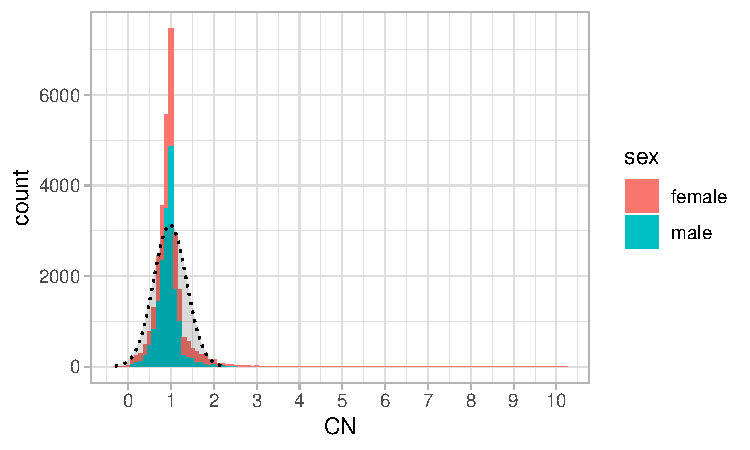
\includegraphics[width=0.58\textwidth]{figures/fig_qc_dist_all_1.pdf}
  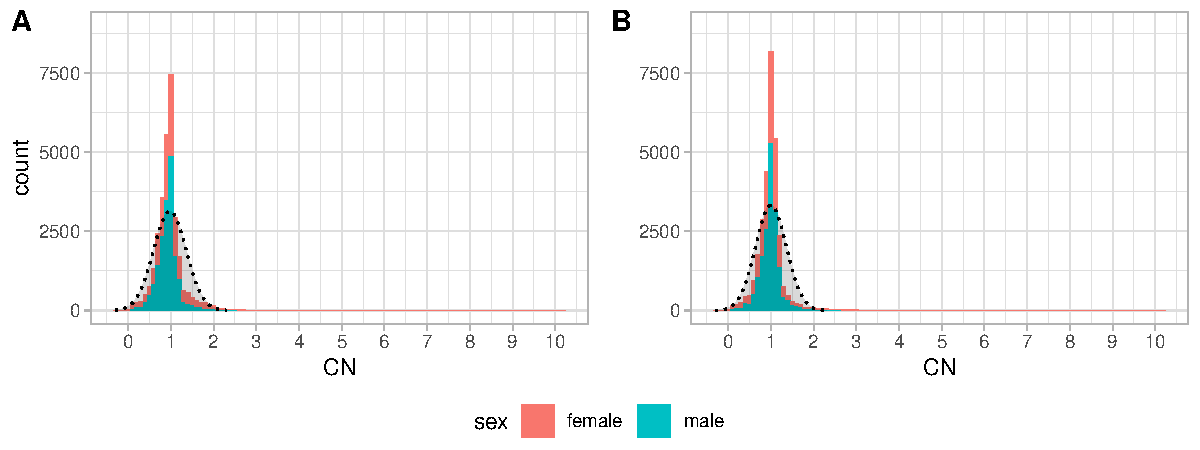
\includegraphics[scale=0.78]{figures/fig_overall_1and3.pdf}
  
  \caption{Distribution of median CN across all genes for all subjects. A normal distribution with an equal median, SD and area (grey) is overlapped as a visual aid. Colored by sexes which are stacked. \textbf{A}: Normalization is achieved through the coverage of the DMD gene. \textbf{B}: Normalization is achieved through shifting the distribution of each individual.}
  
  \label{fig:qc_dist_all}
\end{figure}

The distribution is near symmetrical, centered around a mean of 0.987. This observation lead us to conclude that the normalization of coverage might be achievable using the chromosome wide distribution of copy numbers instead of the DMD coverage. There is no known prior on the chromosome wide copy number distribution. But a mean close to one makes good sense, as it suggests that linked paralogs have been described separately in the annotation.% It also suggests, that the genes in the annotation have a length which is representative of the genomes used in this study.

\noindent We checked that all individuals obey this distribution (figure \ref{fig:qc_subjects_simliki}), and observed that most individuals do. But, Simliki shows a chromosome wide CN median of 1.64, which suggests that Simliki's DMD gene has a size of $ \frac{100\%}{1.64} = 61\%} $ compared to the reference annotation. If using DMD for normalization -- failure to exclude Simliki from subsequent analysis might inflate the CN measurement.
Thus, we decided to carry out the downstream analysis, normalizing the coverage with the assumption that the distribution of all linked genes should have a mean equal to 1. The overall distribution is then as shown in figure \ref{fig:qc_dist_all}B. This assumption carried forward effectively means that the vertical axis in \ref{fig:qc_subjects_simliki} is negatively proportional with the length of the DMD gene in each individual.

%Thus, we decided to remove Simliki from subsequent analysis, and hypothesize, that Simliki's DMD gene might have a deletion. All other individuals have a chromosome wide median CN of less than 1.5, and are thus kept in the downstream analysis.??(fjernelse nævnt to gange) ??overvej også at teste forskel på køn med parret permutationstest.

%Comparing the genes with the highest copy number variation with the results of Lucotte et al





% Figure 2
\begin{figure}[h] 
  \centering
  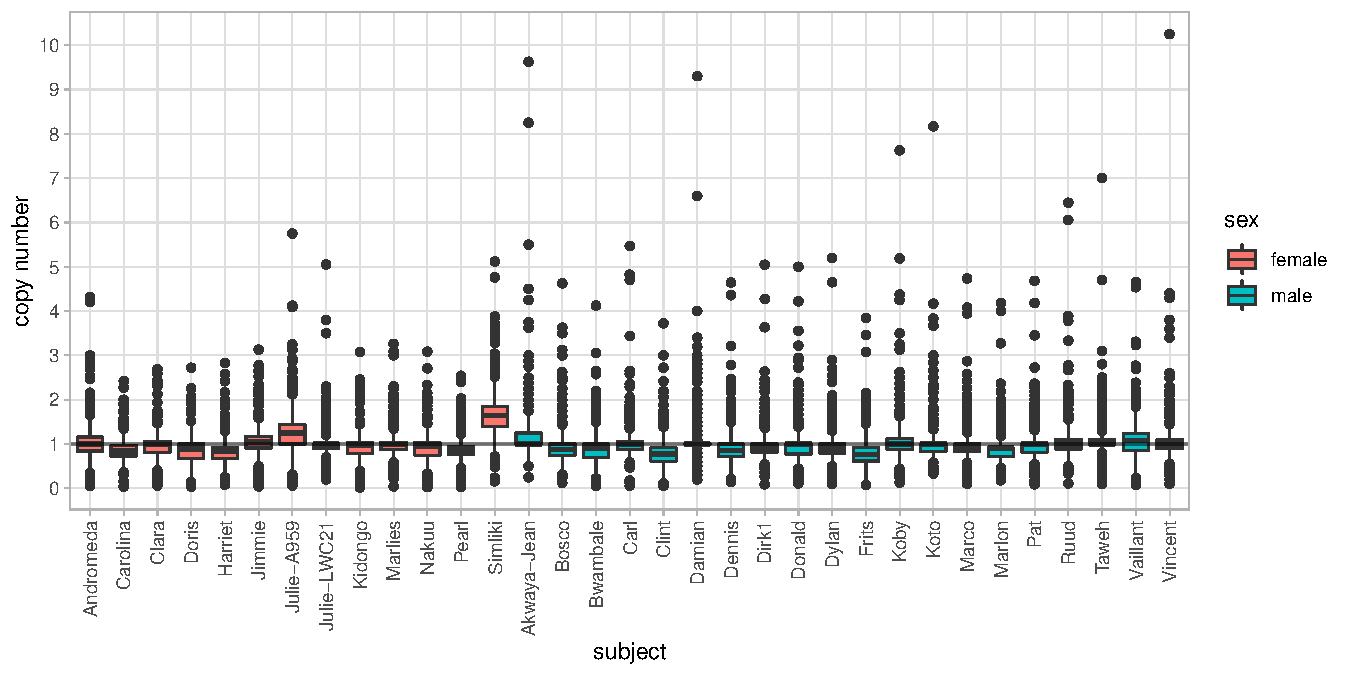
\includegraphics[scale=0.78]{figures/fig_qc_subjects_simliki_1.pdf}
  \caption{Distribution of median CN across all genes for each subject. Coverage normalization is achieved with the coverage of the DMD gene in each individual. Box edges denote quartiles. Points denote values beyond 1.5*IQR, where IQR is the interquartile range.}
  \label{fig:qc_subjects_simliki}
\end{figure}



% Hvorfor er dette interessant?
\noindent Of the 919 genes on the X chromosome, 64 ({\raise.17ex\hbox{$\scriptstyle\sim$}}7\%) have an overlap with another gene. One might suspect that regions where two genes overlap might have a slower turnover than a region with only one gene, because a mutation in one gene will most likely negatively affect the other gene. Nonetheless, performing a non-parametric (permutation) test on the difference (in means) of the distributions of medians for overlapping and non-overlapping genes, shows that the difference is not significant (\textit{p}-value = 0.1927). This means that the copy number variation in the overlap of two genes does not behave differently than a piece of DNA without overlap. 

%\subsection*{Checking paralogs on autosomes}
%In this study, we map the reads to the X chromosome only. Because the rest of the chromosomes might contain paralogs of the genes on the X chromosome, it is relevant to check if the exclusion of the rest of the genome has a significant impact on the coverage of the genes on the X chromosome. In order to check this, we randomly picked a number of individuals (?? which) and compared the coverage of the X chromosome genes from this read mapping, to the read mapping of only the X chromosome. ??results
% Jeg tror ikke jeg kan nå at lave denne sammenligning, desværre. Hellere bruge tiden på at lave en lidt bedre intro.



\subsection*{Most copy number-variant genes}

By measuring the copy number of all genes in all sudjects and focusing on the genes with a median across subjects above 2, we came up with the list of genes enumerated in figure \ref{fig:fig_main}.

% Figure 3
\begin{figure}[h] 
  \centering
  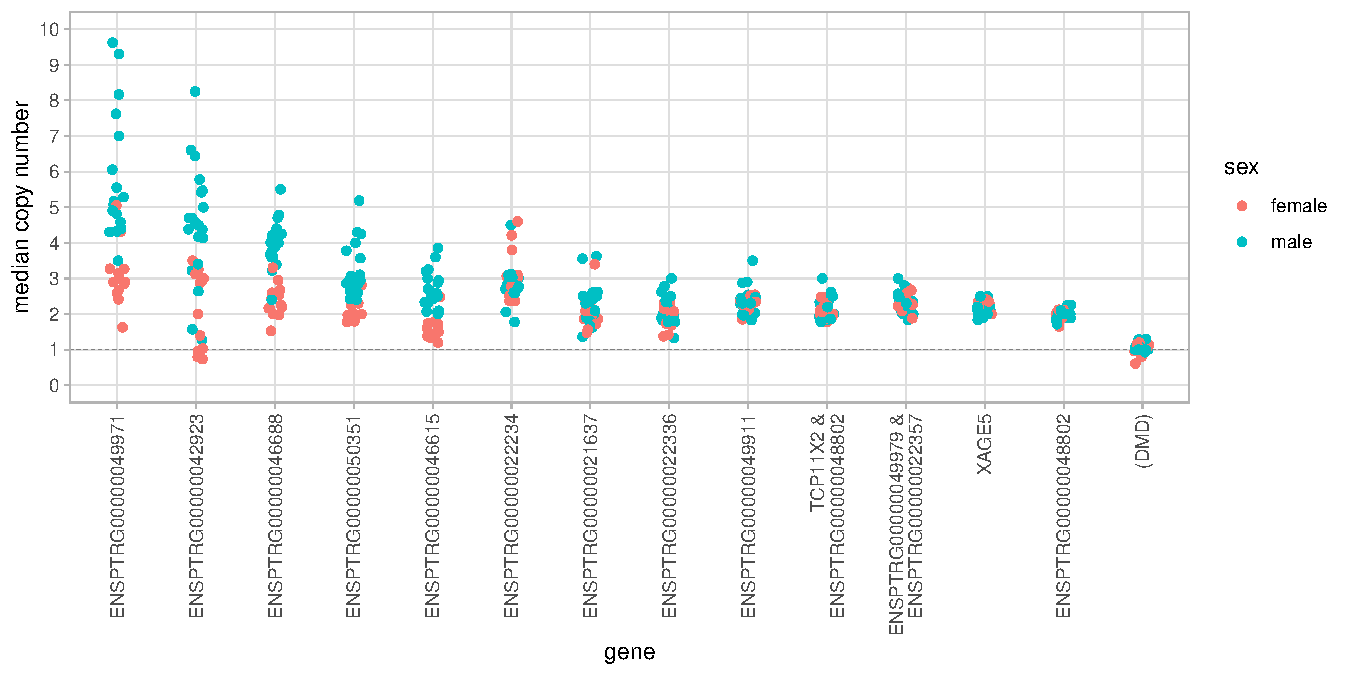
\includegraphics[scale=0.78]{figures/fig_main_3.pdf}
  \caption{Copy number from all subjects, grouped by genes. %These 31 genes or overlaps of genes have a median copy number $\geq$ 1.5. Sorted by descending median. '\&' signifies the overlap of two genes. Horizontal jitter is applied. }
  These 13 genes or overlaps of genes have a median copy number $\geq$ 2. Sorted by descending standard deviation. '\&' signifies the overlap of two genes. Horizontal jitter is applied. DMD is showed for comparison. }
  \label{fig:fig_main}
\end{figure}

Many of the genes with high median copy number show a strong grouping between sexes. This might be because the reads from the X degenerate region on the Y chromosome\cite{skaletsklyMSY} in these males have erroneously mapped to its counterpart on the reference X chromosome. 
As a test, one of the most sexually grouped genes (E..46688) was blast-aligned to the Y chromosome with no matches, which suggests that the sex-grouping is not due to methodological errors. However, because the proportion of sexes in each subspecies is varying (table \ref{tab:subjects}), we have chosen to not to delve further into this clustering, other than noting that something curious is going on. 

We looked up the 13 genes (listed in figure \ref{fig:fig_main}) with the highest SD median copy numbers, where the median is above 2. Unfortunately, many of the genes in the Pan\_tro\_3 reference genome are not named as exhaustively as in the human counterparts which means that many of the genes have serial numbers (ensembl gene ids) instead. These will be abbreviated as ENSPTRG00000049971 to E..49971. 

The genes with the highest median: E..49971 and E..42923 are both related to the 40S ribosomal subunit \cite{ensembl}. Unfortunately, no expression data is available, neither for orthologs.


E..50351 has very sparse information and no ortholog exists in human. A blast search against the human genome identifies a 99\% identical sequence of length $\sim$1900 bp which has expression in many tissues but highest in ovary and testis \cite{ensembl}. 

E..46615 and E..49911 have no description or information about orthologs.

E..22234 "rhox homeobox family member 2" has an ortholog in human: RHOXF2. In human, this gene is expressed in many tissues with the highest levels in testis. It is described as being expressed in early stage germ cells, type-B spermatogonia and early spermatocytes. It has variants that are linked to infertility \cite{10.1093/hmg/ddw313}.

E..21637 is an otherwise uncharacterized gene increasingly expressed in the following organs in order: cerebellum, kidney, prefrontal cortex and testis. In the adult Chimpanzee, this gene is 3 times more expressed in the testis than in any other organ \cite{bgee_}.

E..22336 has no description, but is expressed in the heart and mostly in the testis \cite{bgee_}.

TCP11X2 "t-complex" \& E..48802 is an overlap. TCP11X2 is present in the Pan\_tro\_3 reference genome in two copies (orthologs), which might inflate its copy number. Interestingly the overlap with the gene E..48802 has a higher copy number than the TCP11X2 gene itself. TCP11X2 is not testis expressed \cite{ensembl} but E..48802 is.

The next region which is an overlap of E..49979 \& E..22357. E..49979 is a "heat shock transcription factor" and E..22357 is an otherwise undescribed gene with expression in kidneys.

XAGE5 "X antigen fam. 5" is expressed in cerebellum and mostly testis \cite{bgee_}.

Overlapping the genes from this study with the ones in Lucotte \textit{et al.} 2018 \cite{Lucotte907}, only two genes are present in the top 30 most copy number-variant genes. The first one is OPN1LW which codes for long-wavelength opsin in the retina. Nonetheless, it has its highest expression (in Chimpanzee) in the testis\cite{bgee_}. The other gene, CT47A, presumably orthologous to ENSPTRG00000046894 "cancer/testis antigen 47A" has a max CN of 1.8 and a median CN of 0.9, and is thus not as variant in chimpanzee as in human (human max CN: 15.07, human median CN: 5.01). The other genes deemed copy number-variant in Lucotte \textit{et al.} 2019\cite{Lucotte907} do not have identically named genes in the Chimpanzee annotation.


% We looked up the 30 genes with the highest median copy numbers. Unfortunately, many of the genes in the Pan\_tro\_3 reference genome are not named as exhaustively as in the human counterparts, and many of the genes thus have serial numbers instead. These serial numbers will be abbreviated as ENSPTRG00000049971 to E..49971. 
% The genes with the highest median copy numbers are enumerated in figure \ref{fig:fig_main}.
% \noindent
% E..49971, E..42923, E..46688,  E..22234, E..50351, E..49979, E..46615, E..49911, E..47182, E..48376, E..50450, E..49942, POLA1
% have no obvious relation to anything meiosis related by name or description, and there is no expression data available.
% 
% E..22357, XAGE5, E..22336,  is testis expressed but has no other description.
% 
% E..21637 and OPN1LW have expression in several organs, where testis has the highest.
% 
% EDA, FGF13 and E..41347 is expressed in several organs as well as the testis. TCP11X2, E..23212, TEX28 are testis expressed but has no other description. For E..48802, no Chimpanzee data is related, but an mRNA of an ortholog in Macaca Fascicularis is testis expressed. SPANXN5 has no expression data, but its description "Sperm protein associated with the nucleus on the X chromosome N1" suggests that it is expressed in the testis. ETDB has an identical homolog which is termed "Embryonic testis differentiation homolog", and thus suggests testis expression. E..52876 and E..16737 have no Chimpanzee expression data, but an ortholog in human with an identity of 90\% is testis expressed. E..28324 is not present in all subjects for unknown reasons. Nevertheless, has a median above 1.5, and is testis expressed.
% \noindent Of the genes described in Lucotte et al. 2019, only {\footnotesize OPN1LW} is overlapping as a copy number-variant gene. Even though it codes for long-wavelength opsin in the retina, it has its highest expression in the testis according to the Bgee database (in Chimpanzee). Of the other genes in deemed copy number-variant Lucotte et al. 2019 - CT47A, presumably orthologous to ENSPTRG00000046894 "cancer/testis antigen 47A" has a max CN of 1.8 and a median CN of 0.9, and is thus not as variant in chimpanzee as in human (max CN: 15.07, median CN: 5.01). The other genes deemed copy number-variant in Lucotte et al. 2019 do not have identically named genes in the Chimpanzee annotation.
% That is, assuming that the naming of the genes across the species is completely parsimonous. An alignment is necessary to be able to conclude that these are in fact orthologs.
% \\


\noindent It seems like there is a relation between the high median CN and testis presence. As we don't know what proportion of the X-linked genes are expressed in the testis, it is hard to say if the genes with the highest variation are significantly more present in the testis. Nevertheless, for the genes where expression data was available, all genes but E..22357 showed signs of presence in the testis. More genes with high copy number variation but lower standard deviations than the previously discussed can be found in table \ref{tab:genes}.


\subsection*{Copy number variation among relatives}
The copy number of a gene in a female individual (XX) is the average of the copy number of the two X chromosomes present in its genome. In male individuals (XY), the copy number is the number on the lone X chromosome. This means that by investigating the copy number amongst relatives, we can infer the probable transmission of X chromosomes. Especially in a dad-daughter relation, we know that the copy number of the X chromosome is passed to the daughter. When this daughter then has many sons, it is possible to infer the copy number variation which has occurred meanwhile.

In order to investigate the copy number turnover between parents and offspring, we plotted the copy number over time measured in generations. For 7 of the 33 Chimpanzees included in this study, we know the parent relation, and for 3 we know the grandparent relation. This means that we can compare the progression of copy numbers, down through 2 generations. In figure \ref{fig:pedigree_CN}, the copy numbers for the 6 most highly copied genes is visualized. Dad-son relations are removed because no X chromosome is passed in this relation.

% Figure 4
\begin{figure}[h] 
  \centering
  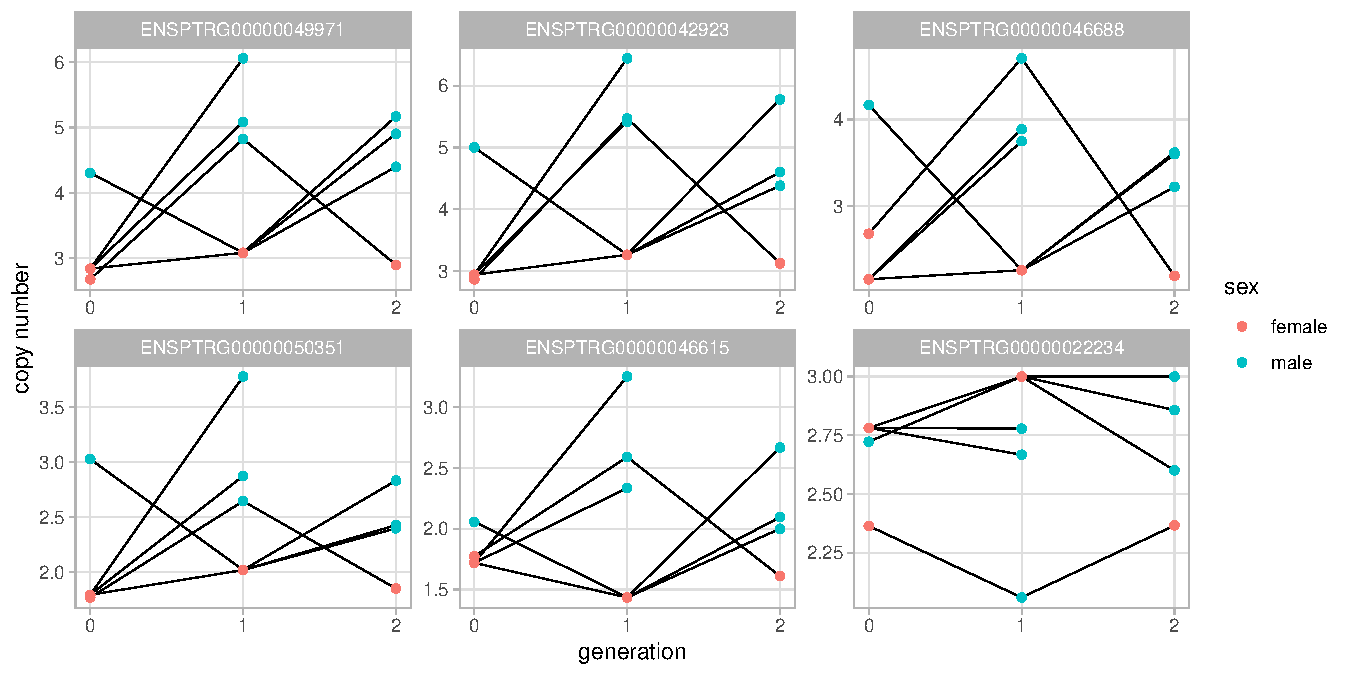
\includegraphics[scale=0.78]{figures/fig_pedigree_CN_3.pdf}
  \caption{Copy number as a function of pedigree. Each straight line denotes the change in copy number for an X-linked gene, when the X chromosome is passed from parent to offspring. Dad-son relations are not included.}
  \label{fig:pedigree_CN}
\end{figure}

Because the sample size of each parent-offspring event is limited, it is impossible to conclude anything on the copy number variation between the generations. Anyhow, For E..49971 there is a parents-daughter relation from generation 0 to 1. Because the daughter has one X from her dad (copy number = 4.3) and one copy from her mom (either copy number = 6 or copy number = 1, as evident from her other sons where the dad is not known and not relevant). Nonetheless, this daughter has three sons with copy numbers = 4.3, 4.9 and 5.1 respectively. It is implicitly given that the X chromosomes in these three sons are the same, and the amount of variation in these sons show that the copy number variation in this gene is not stagnant.




%For E..49971 there is a parents-daughter trio from 0'th to 1'st generation. The mom in this relation also has a son with a high (copy number = 6), which means that this mom will need to have another X chromosome with a copy number correspondingly low around the average of $\sim$3. Because the daughter in the previously mentioned trio repræsents the average of the father (copy number = 4.3) and mom (copy number either 

A similar line of thought can be applied to some of the other genes, implying that the copy number can vary somewhat between generations. This is of course, assuming that the measurements are robust and not due to random fluctuations introduced by methodological errors.


\section*{Conclusion}

This study has searched for genes related to meiotic drive and found handful of good candidates. For the genes where expression data is present, it seems like there is a relation between high median copy number and testis presence. This might support the hypothesis that there is a relation between CNV and meiotic drive.

There is a clustering of median between sexes in some of the most ampliconic genes. The tendency is that males have a higher copy number than females. Though this might be a signal, nothing has been concluded or hypothesized from it. Whether it stems from reads from the X degenerate region on the Y chromosome can be investigated be concatenating the X and Y chromosomes together and checking whether the clustering vanishes. A different and much more interesting act, would be to propose that there is a link between high copy numbers of these genes, and the segregation of a Y chromosome to the sperm cell, leading to male individuals with high copy numbers. It might also be due to random fluctuations.

E..22234, E..21637 and ?? might be good candidates of genes involved in meiotic drive processes. Expression data is missing on the three most wildly copied genes (E..49971, E.46688, E..42923), which might also have a testis-relation.

For many of the genes where identical sequnces are found in other species (mostly human) where testis expression is present, it is not yet investigated whether the ampliconic region is identical to the ortholog or not.

This study has found a handful of genes with high copy number variation which are expressed in the testis. Though some of the genes had no description or expression data available, it seems like most of the most copy variant genes are testis related.
\\
\\
\\

?? Relate to meiotic drive. Give ideas to further analysis.

?? Læs bachproj igen og få ideer.

?? fejlkilder

??Using decoy genome to get rid of paralogs.




\bibliography{sample}

\newpage
\subsection*{Appendix}


\begin{table}[h]
\centering
\begin{tabular}{|l|l|l|l|}
\hline
\textbf{Subject} & \textbf{Sex} & \textbf{Species} & \textbf{Source} \\
%\textbf{Source} & \textbf{Subject} & \textbf{Species} & \textbf{Sex} \\

\hline
%Prado-Martinez et al. 2014  &  Julie-LWC21  &  Pan troglodytes ellioti  &  female  \\
%Prado-Martinez et al. 2014  &  Akwaya-Jean  &  Pan troglodytes ellioti  &  male  \\
%%Prado-Martinez et al. 2014  &  Banyo  &  Pan troglodytes ellioti  &  female  \\
%%Prado-Martinez et al. 2014  &  Basho  &  Pan troglodytes ellioti  &  male  \\
%Prado-Martinez et al. 2014  &  Damian  &  Pan troglodytes ellioti  &  male  \\
%%Prado-Martinez et al. 2014  &  Kopongo  &  Pan troglodytes ellioti  &  female  \\
%Prado-Martinez et al. 2014  &  Koto  &  Pan troglodytes ellioti  &  male  \\
%%Prado-Martinez et al. 2014  &  Paquita  &  Pan troglodytes ellioti  &  female  \\
%Prado-Martinez et al. 2014  &  Taweh  &  Pan troglodytes ellioti  &  male  \\
%%Prado-Martinez et al. 2014  &  Tobi  &  Pan troglodytes ellioti  &  female  \\
%Prado-Martinez et al. 2014  &  Andromeda  &  Pan troglodytes schweinfurthii  &  female  \\
%Prado-Martinez et al. 2014  &  Harriet  &  Pan troglodytes schweinfurthii  &  female  \\
%Prado-Martinez et al. 2014  &  Kidongo  &  Pan troglodytes schweinfurthii  &  female  \\
%Prado-Martinez et al. 2014  &  Nakuu  &  Pan troglodytes schweinfurthii  &  female  \\
%Prado-Martinez et al. 2014  &  Bwambale  &  Pan troglodytes schweinfurthii  &  male  \\
%Prado-Martinez et al. 2014  &  Vincent  &  Pan troglodytes schweinfurthii  &  male  \\
%Prado-Martinez et al. 2014  &  Clara  &  Pan troglodytes troglodytes  &  female  \\
%Prado-Martinez et al. 2014  &  Doris  &  Pan troglodytes troglodytes  &  female  \\
%Prado-Martinez et al. 2014  &  Julie-A959  &  Pan troglodytes troglodytes  &  female  \\
%Prado-Martinez et al. 2014  &  Vaillant  &  Pan troglodytes troglodytes  &  male  \\
%Prado-Martinez et al. 2014  &  Jimmie  &  Pan troglodytes verus  &  female  \\
%Prado-Martinez et al. 2014  &  Bosco  &  Pan troglodytes verus  &  male  \\
%Prado-Martinez et al. 2014  &  Clint  &  Pan troglodytes verus  &  male  \\
%Prado-Martinez et al. 2014  &  Koby  &  Pan troglodytes verus  &  male  \\
%Prado-Martinez et al. 2014  &  Donald  &  Pan troglodytes verus x troglodytes  &  male \\
%Besenbacher et al. 2019  &  Carolina  &  Pan troglodytes verus  &  female  \\
%Besenbacher et al. 2019  &  Simliki  &  Pan troglodytes verus  &  female  \\
%Besenbacher et al. 2019  &  Carl  &  Pan troglodytes verus  &  male  \\
%Besenbacher et al. 2019  &  Frits  &  Pan troglodytes verus  &  male  \\
%Venn et al. 2014  &  Pearl  &  Pan troglodytes verus  &  female  \\
%Venn et al. 2014  &  Marlies  &  Pan troglodytes verus  &  female  \\
%Venn et al. 2014  &  Marco  &  Pan troglodytes verus  &  male  \\
%Venn et al. 2014  &  Dirk1  &  Pan troglodytes verus  &  male  \\
%Venn et al. 2014  &  Dennis  &  Pan troglodytes verus  &  male  \\
%Venn et al. 2014  &  Ruud  &  Pan troglodytes verus  &  male  \\
%Venn et al. 2014  &  Dylan  &  Pan troglodytes verus  &  male  \\
%Venn et al. 2014  &  Marlon  &  Pan troglodytes verus  &  male  \\
%Venn et al. 2014  &  Pat  &  Pan troglodytes verus  &  male  \\









Julie-LWC21  &  female  &  Pan troglodytes ellioti  & Prado-Martinez et al. 2014  \\
Akwaya-Jean  &  male  &  Pan troglodytes ellioti  & Prado-Martinez et al. 2014  \\
%Banyo  &  female  &  Pan troglodytes ellioti  & %Prado-Martinez et al. 2014  \\
%Basho  &  male  &  Pan troglodytes ellioti  & %Prado-Martinez et al. 2014  \\
Damian  &  male  &  Pan troglodytes ellioti  & Prado-Martinez et al. 2014  \\
%Kopongo  &  female  &  Pan troglodytes ellioti  & %Prado-Martinez et al. 2014  \\
Koto  &  male  &  Pan troglodytes ellioti  & Prado-Martinez et al. 2014  \\
%Paquita  &  female  &  Pan troglodytes ellioti  & %Prado-Martinez et al. 2014  \\
Taweh  &  male  &  Pan troglodytes ellioti  & Prado-Martinez et al. 2014  \\
%Tobi  &  female  &  Pan troglodytes ellioti  & %Prado-Martinez et al. 2014  \\
Andromeda  &  female  &  Pan troglodytes schweinfurthii  & Prado-Martinez et al. 2014  \\
Harriet  &  female  &  Pan troglodytes schweinfurthii  & Prado-Martinez et al. 2014  \\
Kidongo  &  female  &  Pan troglodytes schweinfurthii  & Prado-Martinez et al. 2014  \\
Nakuu  &  female  &  Pan troglodytes schweinfurthii  & Prado-Martinez et al. 2014  \\
Bwambale  &  male  &  Pan troglodytes schweinfurthii  & Prado-Martinez et al. 2014  \\
Vincent  &  male  &  Pan troglodytes schweinfurthii  & Prado-Martinez et al. 2014  \\
Clara  &  female  &  Pan troglodytes troglodytes  & Prado-Martinez et al. 2014  \\
Doris  &  female  &  Pan troglodytes troglodytes  & Prado-Martinez et al. 2014  \\
Julie-A959  &  female  &  Pan troglodytes troglodytes  & Prado-Martinez et al. 2014  \\
Vaillant  &  male  &  Pan troglodytes troglodytes  & Prado-Martinez et al. 2014  \\
Jimmie  &  female  &  Pan troglodytes verus  & Prado-Martinez et al. 2014  \\
Bosco  &  male  &  Pan troglodytes verus  & Prado-Martinez et al. 2014  \\
Clint  &  male  &  Pan troglodytes verus  & Prado-Martinez et al. 2014  \\
Koby  &  male  &  Pan troglodytes verus  & Prado-Martinez et al. 2014  \\
Donald  &  male  &  Pan troglodytes verus x troglodytes & Prado-Martinez et al. 2014  \\
Carolina  &  female  &  Pan troglodytes verus  & Besenbacher et al. 2019  \\
Simliki  &  female  &  Pan troglodytes verus  & Besenbacher et al. 2019  \\
Carl  &  male  &  Pan troglodytes verus  & Besenbacher et al. 2019  \\
Frits  &  male  &  Pan troglodytes verus  & Besenbacher et al. 2019  \\
Pearl  &  female  &  Pan troglodytes verus  & Venn et al. 2014  \\
Marlies  &  female  &  Pan troglodytes verus  & Venn et al. 2014  \\
Marco  &  male  &  Pan troglodytes verus  & Venn et al. 2014  \\
Dirk1  &  male  &  Pan troglodytes verus  & Venn et al. 2014  \\
Dennis  &  male  &  Pan troglodytes verus  & Venn et al. 2014  \\
Ruud  &  male  &  Pan troglodytes verus  & Venn et al. 2014  \\
Dylan  &  male  &  Pan troglodytes verus  & Venn et al. 2014  \\
Marlon  &  male  &  Pan troglodytes verus  & Venn et al. 2014  \\
Pat  &  male  &  Pan troglodytes verus  & Venn et al. 2014 \\
\hline

\end{tabular}
\caption{\label{tab:subjects}Metadata for the 33 subjects used in this study.}
\end{table}










\end{document}